\documentclass{TUBAFarbeiten}
\usepackage{graphics}
\usepackage{wrapfig}
\usepackage{listings}
\usepackage{xcolor}
\usepackage[utf8]{inputenc}
\usepackage[nottoc,numbib]{tocbibind}
\usepackage{tikz}

\newcommand{\lstin}[1]{\lstinline[language=C]{#1}}

\lstdefinestyle{customc}{
  belowcaptionskip=1\baselineskip,
  breaklines=true,
  frame=L,
  xleftmargin=\parindent,
  language=C,
  showstringspaces=false,
  basicstyle=\footnotesize\ttfamily,
  keywordstyle=\bfseries\color{green!40!black},
  commentstyle=\itshape\color{purple!40!black},
  identifierstyle=\color{blue},
  stringstyle=\color{orange},
}

\TUBAFFakultaet{Fakultät für Mathematik und Informatik}
\TUBAFInstitut{Institut für Informatik}

\TUBAFTitel{Exploring Data Structures in C | Skip List}
\TUBAFAutor[F. Bär]{Fabian Bär}
\TUBAFStudiengang{Angewandte Informatik}
\TUBAFMatrikel{64762}
\begin{document}
\maketitle
\tableofcontents
\newpage

\section{Vorwort}
In dieser Arbeit wird die Datenstruktur Skip List vorgestellt. Diese soll Einträge, bestehend aus Schlüssel und Wert speichern. Es sollen diese zeiteffizient eingefügt und gesucht werden können. Die Funktionalität findet viele Anwendungen in der Programmierung, zum Beispiel in Datenbanken. Eine Implementation der Datenstruktur und die Fragestellung, ob die Skip List zeiteffizient genug ist, ist Inhalt dieser Arbeit.

\section{Grundlegendes}
Die Skip List ist eine geordnete Assioziative \cite{itvis} Datenstruktur.  Wie in einer Linked List, verweist ein Element jeweils auf das nächste. Zusätzlich können weiter entfernte Elemente verlinkt sein, um einen schnelleren Zugriff zu ermöglichen. Die Skip List hat beim Suchen, Überschreiben, Einfügen und Entfernen die Zeitkomplexität von
 \(O(log(n))\).
In einer Skip List können Elemente, die aus Schlüssel und Wert bestehen eingefügt, gesucht und entfernt werden. 
Die Skip List besteht aus Schichten. In der untersten Schicht zeigt jedes Element auf das nachfolgende. In den darüber liegenden Schichten können Elemente übersprungen werden. Ein Element kann zum Beispiel auf das übernächste zeigen, jedoch ist dies nur erlaubt, wenn der Eintrag auch in der Schicht darunter existiert.
\begin{wrapfigure}{l}{0.55\textwidth}
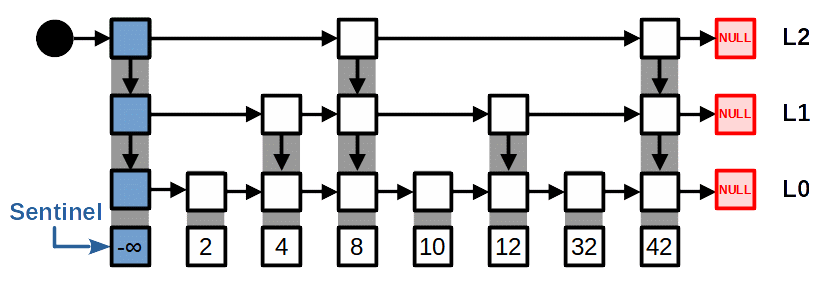
\includegraphics[scale=0.3]{img/aufbau1}
\caption{Aufbau einer Skip List}
\label{fig:Img1}
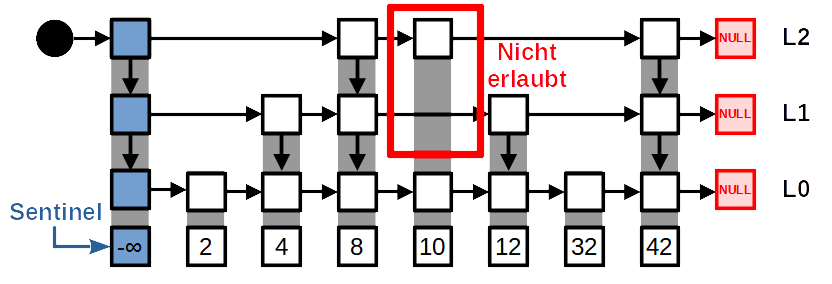
\includegraphics[scale=0.3]{img/aufbau1_falsch}
\caption{Nich korrekter Aufbau einer Skip List}
\label{fig:Img2}
\end{wrapfigure}
Die Skip List kann man als gerichteten Graphen modellieren, wobei ein Knoten jeweils einem Element und einer Schicht zugeordnet ist. Die von dort ausgehenden Kanten können auf den Knoten der darunterliegenden Schicht des selben Elements; und auf den Knoten des folgenden Elements auf der selben Schicht zeigen, wobei die Kanten Information über die Richtung ( "`Schicht runter"', "`nächstes auf selber Schicht"') enthalten. Es ist sinnvoll, dass das erste ein so genanntes Sentinel-Element ist, welches in der höchsten Schicht ist. \cite{suswang}1:36 In den vom Nutzer ausgeführten Operationen wird dieses ignoriert. Die Sentinel erleichtert die Algorithmen, da diese immer ganz am Anfang der Liste steht und daher keine Fallunterscheidung getroffen werden muss, ob am Anfang hinzugefügt oder entfernt wird. 
Für den Folgenden Absatz wird angenommen, dass s die Höhe einer Schicht ist. Für die unterste Schicht wäre \(s = 0\), für die Schicht darüber \(s = 1\) und so weiter.
Für den idealen Aufbau der Skip List der Länge n solte die Anzahl der Knoten pro Schicht \(ld(s) \cdot n\) und die Abstände zwischen den Knoten einer Schicht möglichst ähnlich sein. 

\section{Operationen}

\subsection{Anzahl der Elemente ermitteln}

Um die Anzahl der Elemente (Senitnel ausgenommen) zu ermitteln, wird bei dem Knoten auf der untersten Schicht der Sentinel begonnen. Es wird solange die Kante "`nächstes auf selber Schicht"' zum nächsten Knoten gegangen, bis diese nicht mehr existiert. Die Anzahl der gegangenen Kanten entspricht der Länge der Liste und der Anzahl der Elemente.  Die Zeitkomplexität wäre \(O(n)\).
Alternativ kann die Anzahl der Elemente auch als Zahl mit gespeichert werden und beim Einfügen eines Elementes inkrementiert und beim Entfernen dekrementiert werden. Mit dieser Methode ist die Zeitkomplexität beim Auslesen für die Operation \(O(1)\).

\subsection{Suchoperation}

Die Suchoperation gitb das Element mit dem gesuchten Schlüssel zurück, falls es existert.
Begonnen wird mit dem Knoten auf der obersten Schicht des Sentinels.\\
1.: Wenn der gesuchte Schlüssel gleich dem Schlüssel des dem Knoten zugehörigen Elements ist, wurde das Element gefunden und kann zurück gegeben werden. Falls die Schlüssel ungleich sind, wird der nächte Knoten auf der selben Ebene betrachtet.\\
2.: Wenn dieser nicht existiert oder deren Schlüssel nach dem des gesuchten Schlüssels liegt, wird zurück zu dem Knoten in Schritt 1 gegangen, sonst Schritt 1 mit dem gerade betrachteten Knoten ausgeführt.\\
3.: Es wird eine Ebene herunter gegangen. Wenn die Ebene darunter nicht existiert, existiert das gesuchte Element nicht und es wird zurück gegeben, dass das Element mit dem gesuchten schlüssel nicht existiert. Sonst wird Schritt 1 wieder ausgeführt.

\subsection{Überschreibeoperation}

Die Überschreibeoperation ändert den Wert des eines bereits existierenden Elements mit einem bestimmten Schlüssel.
Es wird eine Suchoperation ausgeführt. Das Wert-Feld des zurückgegebenen Elements wird auf den neuen Wert gesetzt.

\subsection{Einfügeoperation}

Die Einfügeoperation fügt ein neues Element mit einem bestimmten Schlüssel hinzu. Es existiert vorher kein Element mit diesem Schlüssel in der Liste.
Bis zu welcher Ebene eingefügt wird ist zufällig. Durch die Zufälligkeit nähert sich die die Skip List im Aufbau der idealen Skip List an, jedoch kann es auch für einige Zufallsergebnisse deutlich schlechter sein. Dies wird im Abschnitt Zeitkomplexität und in den Geschwindigkeitstests weiter erläutert. \\
Es wird eine Suchoperation (die fehlschlägt) ausgeführt, jedoch werden die aktuellen Knoten in Schritt 3 der Suchoperation in einer Liste gespeichert.
Die "`nächstes auf selber Schicht"' Kanten dieser Knoten würden das neue Element überspringen. Zwischen dem und dem nächsten würden die Knoten des neuen Elementes eingefügt werden. \\ 1.: Das neue Element wird erstellt. \\ 2.: Auf der untersten Schicht wird ein Knoten erstellt und eingefügt. Da beim Suchen Knoten gespeichert wurden, deren Kanten die Position überspringen, ist bekannt wo er eingefügt werden muss. \\ 3.: Mit einer Wahrscheinlichkeit von 50\% wird ein Knoten auf der Schicht darüber eingefügt, sonst wird abgebrochen. Existert die Schicht noch nicht, wird eine neue Schicht erstellt und ebenfalls an der Sentinel ein Knoten dieser Schicht eingefügt. \\ 4.: Schritt 3 wird erneut ausgeführt.

\subsection{Entfernoperation}

Die Entfernenoperation löscht ein extistierendes Element mit einem bestimmten Schlüssel aus der Liste.
Es wird eine Suchoperation, mit dem Schlüssel minimal kleiner als der Gesuchte ausgeführt (dieser darf kein Element finden). Wie beim Einfügen werden die Knoten gespeichert, deren "`nächstes auf selber Schicht"' Kanten das zu entfernende Element überspringen. Diese Knoten sind die Vorgänger der Knoten des zu entfernenden Elements, vorrausgesetzt auf selber Schicht existert ein Knoten des zu entfernenden.
Dann wird eine Suchoperation für das zu entfernende Element durchgeführt und der oberste Knoten dieses mit gespeichert.
Die Nachfolgerkanten der gespeicherten Vorgänger werden mit den Nachfolgerkanten der Knoten auf selber Schicht des zu entfernenden Elements überschrieben, wenn sie existieren.

\section{Zeitkomplexität}

Die Zeitkomplexität für die Suchoperation beträgt \(O(log(n))\).
Zunächst wird eine ideale Skip List mit der Länge \(n = 2 ^ k\) (inklusive Sentinel) betrachtet, wobei k die Anzahl der Schichten ist. In der Folgenden Abbildung ist eine solche Skip List mit \(k = 3\) dargestellt. 
\begin{wrapfigure}{l}{0.6\textwidth}
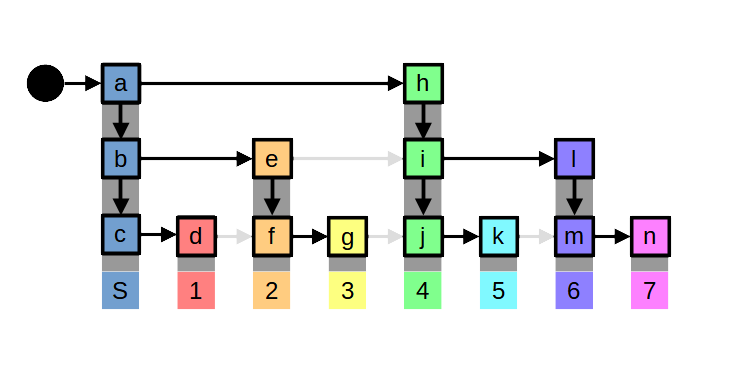
\includegraphics[scale=0.4]{img/ideal}
\caption{Ideale Skip List mit k=3. Die für den Suchvorgang nicht verwendeten Kanten sind grau dargestellt.}
\label{fig:Img3}
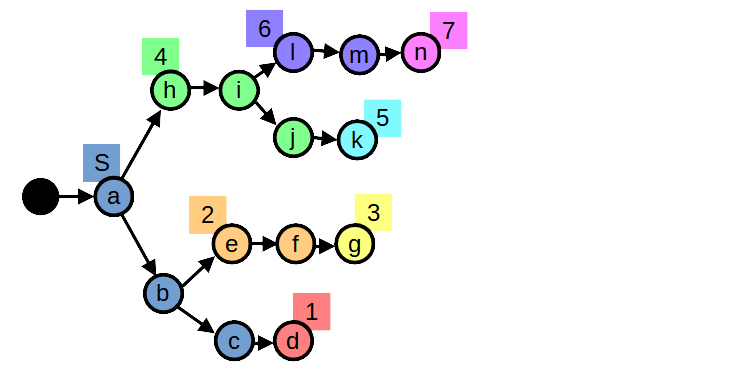
\includegraphics[scale=0.4]{img/ideal_baum}
\caption{Binärbaum}
\label{fig:Img4}
\end{wrapfigure}
Entfernt man die im Suchvorgang nicht verwendeten Kanten, entsteht ein Binärbaum. Der längste Weg ist der zum letzten Element. Dieser ist l = \(2 \cdot k\) Knoten lang, da k mal abwechselnd weiter auf selber Ebene und nach unten gegangen werden muss. Daraus folgt, dass \(l = ld(n)\). Somit hat dieser Zugriff eine Zeitkomplexität von \(O(log(n))\). 

Es lässt sich beweisen, dass mit hoher Wahrscheinlichkeit die Suche in einer zufällig aufgebauten Skip List auch eine Zeitkomplexität von \(O(log(n))\) hat. \cite{mitocw}1:07:00
Bei sehr ungünstigen Zufallsergebnissen kann es jedoch dazu kommen, dass die Anzahl der Schichten fast unendlich groß ist (es kam zufällig sehr oft hintereinander "`Schicht erhöhen"' heraus). In diesem Fall dauert die Suche deutlich länger. Es kann auch sein, dass die Liste nur aus einer Schicht besteht. Das ist der Fall, wenn  nur "`Schicht nicht erhöhen"' gewürfelt wird. In diesem Fall entsteht eine Linked List mit einer Suchzeitkomplexität von \(O(n)\). In der Realität passiert dies aber sehr selten, jedoch können diese Effekte auch in Teilen der Liste auftreten, zum Beispiel, dass viele aufeinander folgende Elemente nur der untersten Schicht existeren.

\section{Implementation in C}

\subsection{list element.h}
In \lstin{list_element.h} sind die Struktur, bestehend aus Schlüssel und Wert, sowie die dazugehörigen Schlüssel- und Wert-Datentypen und die Schlüsselvergleichsoperation definiert.
Die Definition der Schlüssel- und Wert-Datentypen efolgt durch die Makros \lstin{LIST_KEY_TYPE} und \lstin{LIST_VALUE_TYPE}. Beide werden mit int definiert. \lstin{LIST_VALUE_NOT_FOUND} wird zurück gegeben, wenn der Wert eines nicht existierenden Elements angefragt wird. \\ \lstin{LIST_KEY_COMPARE(targetKey, checkKey)} gibt eine negative Zahl zurück, wenn targetKey nach checkKey eingeordnet ist, eine positive, wenn es umgekehrt ist, und 0, wenn die Schüssel identisch sind. 

\subsection{skip list.h}
In \lstin{skip_list.h} ist die Struktur \lstin{skip_list} und \lstin{skip_list_node} definiert.
\lstin{skip_list} speichert einen Pointer auf den Sentinel-Knoten der obersten Schicht und hat Felder für die Länge der Liste (ohne Sentinel) und die Anzahl der Schichten.
Die Datenstruktur \lstin{skip_list_node} enthält Pointer zu dem nächsten Knoten auf selber Ebene und den darunter liegenden Knoten. Existieren diese nicht, ist das Feld auf null gesetzt. Die Datenstruktur enthält auch einen Pointer auf das zugehörige List-Element.
In der Datei sind zudem alle Funktionsköpfe Definiert. Auf die Funktionen wird im Abschnitt Funktionen eingegangen.

\subsection{skip list.c}
In \lstin{skip_list.c} sind die Funktionen implementiert.

\subsection{Funktionen}

\subsubsection{\lstin{skip_list__init}}

\lstin{void skip_list__init(skip_list_t* list)} \\

Diese Funktion initialisiert die übergebene Liste. Es wird der Sentinel-Knoten für Schicht 0, mit Sentinel-Element erstellt und in der Liste verlinkt. Die Anzahl der Elemente ist 0 und die Anzahl der Schichten ist 1.

\subsubsection{\lstin{skip_list__get_element}}

\lstin{list_element_t* skip_list__get_element(skip_list_t* list, LIST_KEY_TYPE key)} \\

Diese Funktion sucht das Element (Datenstruktur bestehend aus Schlüssel und Wert) in der Liste list mit dem Schlüssel key. Es wird null zurück gegeben, wenn es nicht existiert. 

\begin{lstlisting}[language=C, frame=single, style=customc]
skip_list_node_t* before = list->sentinelTop;
skip_list_node_t* current = before->next;
int delta;
while (1) {
    delta = current == NULL ? -1 : LIST_KEY_COMPARE(key, current->element->key);
    if (delta == 0) return current->element;
    if (delta > 0) {
        // keep on this layer
        before = current;
        current = current->next;
    } else {
        // back, layer down, next
        current = before->down;
        if (current == NULL) return NULL; //layer down not possible
        before = current;
        current = current->next;
    }
}
\end{lstlisting}

before und current sind Variablen, in denen Knoten gespeichert sind.
Am Anfang ist before der oberste Sentinel-Knoten und next sein nachfolge Knoten auf selber Schicht.
Folgendes wird in einer Schleife durchgeführt.
Als erstes wird der Schlüsselvergleich vom current Knoten und dem gesuchten Schlüssel durchgeführt. Wenn current null ist, ist das Ende der Liste auf dieser Schicht erreicht, das gesuchte Element müsste eine Schicht darunter weiter gesucht werden, deshalb wird delta für diesen Fall auf -1 gesetzt.
Wenn die Schlüssel identisch sind, ist das dem current zugehörige Element das gesuchte und wird zurückgegeben.
Sonst wird getestet, ob das gesuchte Element schon übersprungen wurde. Wenn es noch nicht übersprungen wurde (\(delta > 0\)), wird auf dieser Schicht weiter gegangen, sonst wird zurück und dann eine Schicht herunter gegangen. Sollte in diesem Fall current null sein, war das Heruntergehen nicht möglich, da man sich schon auf der untersten Schicht befand. Das gesuchte Element existiert nicht, es wird null zurück gegeben. Sonst wird auf der Schicht noch eins weiter gegangen und dann mit dem nächsten Schleifenduchlauf begonnen.
Die Variable before wird für das zurückgehen benötigt.

\subsubsection{\lstin{skip_list__get}}

\lstin{LIST_VALUE_TYPE skip_list__get(skip_list_t* list, LIST_KEY_TYPE key)} \\

Diese Funktion gibt den Wert des Elements mit dem Schlüssel key in der Skip List list zurück, wenn es existiert, sonst ist der Rückgabewert \lstin{LIST_VALUE_NOT_FOUND}.
Es wird \lstin{skip_list__get_element(list, key)} ausgeführt, wenn deren Rückgabewert ungleich null ist wird der Wert des Elements ausgelesen und zurückgegeben, sonst wird \lstin{LIST_VALUE_NOT_FOUND} zurück gegeben.

\subsubsection{\lstin{skip_list__set}}

\lstin{void skip_list__set(skip_list_t* list, LIST_KEY_TYPE key, LIST_VALUE_TYPE value)} \\

Diese Funktion fügt ein neues Element mit dem Schlüssel key und dem Wert value in die Liste list ein, wenn sich in dieser noch keins mit diesem Schlüssel befindet. Sonst wird der Wert dieses Elements mit value überschrieben.

\begin{lstlisting}[language=C, frame=single, style=customc]
if (skip_list__overshootStack == NULL) skip_list__overshoot_init();
int overshootStackCounter = 0;
skip_list_node_t* before = list->sentinelTop;
skip_list_node_t* current = before->next;
int delta;
while (1) {
    delta = current == NULL ? -1 : LIST_KEY_COMPARE(key, current->element->key);
    if (delta == 0) {
        current->element->value = value;
        return;
    }
    if (delta > 0) {
        // keep on this layer
        before = current;
        current = current->next;
    } else {
        // back, layer down, next
        
        if (overshootStackCounter >= skip_list__overshootStackMaxSize) skip_list__overshoot_larger();
        
		// den Knoten auf den Stapel legen
        skip_list__overshootStack[overshootStackCounter++] = before;
        current = before->down;
        before = current;
        if (current == NULL) {
            // neues element dazwischen schieben
            skip_list_node_t* newNode;
            skip_list_node_t* newNodeBefore = NULL;
            list_element_t* el = skip_list__newElement(key);
            el->value = value;
            do {
                skip_list_node_t* newNode = skip_list__newNode();
                newNode->element = el;
                newNode->down = newNodeBefore;
                if (overshootStackCounter == 0) {
                    // neuer Layer erstellen
                    skip_list_node_t* newSentinelTop = skip_list__newNode();
                    newSentinelTop->down = list->sentinelTop;
                    newSentinelTop->next = newNode;
                    newSentinelTop->element = list->sentinelTop->element;
                    
                    list->sentinelTop = newSentinelTop;
                    
                    newNode->next = NULL;
                    
                    list->_layers++;
                } else {
                    // knoten auf aktueller Schicht neu verbinden
                    overshootStackCounter--;
                    newNode->next = skip_list__overshootStack[overshootStackCounter]->next;
                    skip_list__overshootStack[overshootStackCounter]->next = newNode;
                }
                newNodeBefore = newNode;
            } while (rand() & 1);//50% probabilidy
            list->_size++;
            return;
        }
        skip_list__overshootStack[overshootStackCounter++] = before;
        before = current;
        current = current->next;
    }
}
\end{lstlisting}

Der grundlegende Aufbau ist genaus so, wie der in \lstin{skip_list__get_element}. Zusätzlich wird beim Zurückgehen gespeichert, zu welchen Knoten zurück gegangen wurden. Die von diesen abgehenden Kanten würden die Position überspringen, in die eingefügt wird. Das Speichern der Knoten wird mit einem Stack realisiert, welcher als globale Variable angelegt wurde. Dies ist zu hinterfragen, da Multithreading damit nicht möglich ist. Wird das richtige Element gefunden, muss nur das value-Feld überschrieben werden. Wurde es nicht gefunden wird ein neues Element eingefügt. Als erstes wird das Element erstellt. Dann wird ein Knoten erstellt und in die unterste Schicht, nach dem im Stapel gespeicherten Knoten und vor deren Nachfolger eingefügt. Mit einer Wahrscheinlichkeit von 50 \% wird das selbe für die Schicht darüber wiederholt. Existiert die Schicht noch nicht, wird sie angelegt und das Feld für die Anzahl der Schichten wird inkrementiert. Hierbei muss auch für die Sentinel ein neuer Knoten erstellt und der Zeiger in der Listenstruktur geändert werden. Mit einer Wahscheinlichkeit von 50 \% wird wieder eine neue Schicht hinzugefügt und so weiter. Beim Einfügen wird die Anzahl der Elemente inkrementiert.

\subsubsection{\lstin{skip_list__size}}

\lstin{int skip_list__size(skip_list_t* list)} \\

Gibt die Anzahl der Elemente (ohne Sentinel) der Liste list zurück, in dem das Feld \lstin{_size} ausgelesen wird.

\subsubsection{\lstin{skip_list__layers}}

\lstin{int skip_list__layers(skip_list_t* list)} \\

Gibt die Anzahl der Schichten der Liste list zurück, in dem das Feld \lstin{_layers} ausgelesen wird.

\subsection{Speicher für neue Knoten und Elemente}

Es wurden zwei verschiedene Verfahren implementiert, wo die neuen Knoten und Elemente gespeichert werden. Die erste möglichkeit ist durch Alloziieren von neuen Speicher mittels malloc. Dies hat den Vorteil, dass, solange genug platz auf dem heap ist, neu alloziiert werden kann. Der Nachteil daran ist, dass die Elemente verstreut über den gesammten heap liegen und es dadurch meistens unmöglich ist nachfolgende Knoten gleich mit in den cache zu laden.

Das zweite Verfahren nutzt ein sehr großes globales Array für Elemente und Knoten, welches von vorn nach hinten mit diesen befüllt werden kann. Der Vorteil ist, dass die Knoten in der Nähe voneinander liegen. Der Nachteil ist, dass je nach Länge der Liste entweder sehr viel Speicher ungenutzt ist oder das Array voll ist.

Eine drittes Verfahren wäre Speicherblöcke, in denen Platz für einige Knoten oder Elemente ist, mit malloc zu alloziieren.

\section{Geschwindigkeitstests der Implementation}

Die Skip List Implementationen wurden auf Geschwindigkeit in Abhängigkeit von der sich in der Liste befindenden Elemente getestet. Am Anfang jedes Tests wird eine Skip List mit einmals zufällig generierten Schlüsseln, die in einer Datei gespeichert sind gebaut. Diese Schlüssel sind einzigartig, liegen zwischen 0 und 33554430 und sind gerade.
Dann wird die Zeit in Millsekunden für 1000 such oder einfüge Operationen mit einmals generierten Schlüsseln, die zwischen 1 und 33554431 liegen und ungerade sind gemessen. Diese Schlüssel sind auch in einer Datei gespeichert. 

\subsection {Vergleich Skip List und Liste in Array}

In folgender Grafik sind die Lese- und Einfügezeiten der Skip List in Abhängigkeit von der Länge der Liste und die Lese- und Einfügezeiten einer Listenimplementation mittels Array dargestellt.
In der Array-Implementation werden alle Elemente nacheinander in einem Array gespeicherrt. Beim Suchen wird entweder duch das Array iteriert oder Binärsuche angewendet. Beim Einfügen werden die nachfolgenden Elemente mittels memmove verschoben und gegebenenfalls das Array verlängert (neu alloziiert).

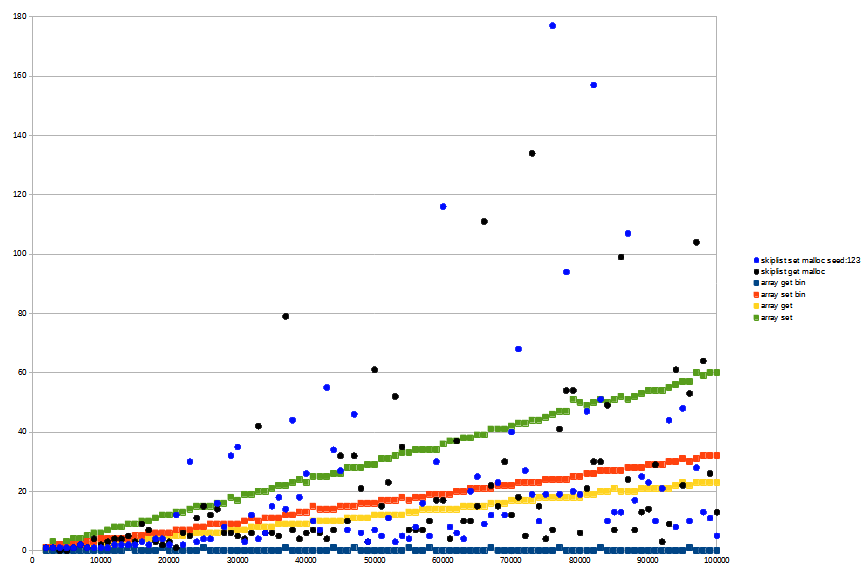
\includegraphics[scale=0.55]{img/diagram_array_skiplist}
\label{fig:Img5}

Die Suche im Array ohne Binär suche scheint Linear zu wachsen \(O(n)\). Die Suche im Array mit Binärsuche ist so schnell, dass sie nicht genau erfasst werden kann. Diese ist vermutlich \(O(log(n))\). Die Einfüge Operationen im Array wachsen Linear, jedoch ist die Binärsuche-Variante schneller, da die Suchzeit deutlich schneller ist. Beide scheinen \(O(n)\) zu sein.
Die Zeiten der Lese- und Schreiboperation in der Skip List scheinen stark zu streuen. Dies könnte am zufälligen Aufbau liegen, da die Skip List mal mehr oder weniger ideal gebaut wird. Im Streuungsmuster kann an erkennen, dass es sich um einen logarithmischen Anstieg handelt. Die Leseoperationen scheinen schneller als die Schreiboperationen zu sein. Dies ist zu erwarten, da die Schreiboperation, wie die Lese Operation die richtige Stelle zum Einfügen suchen muss und zusätzlich das Einfügen der Knoten berechnet werden muss.

\subsection{Einfluss des Zufalls}

Die Randomisierung erfolgt mittels eines Pseudozufallsgenerators, das heißt, dass sich noch mal die selben Zufallszahlen generieren lassen können. Dies wurde genutzt, um den selben Test ein zweites Mal duch zu führen und die Ergebnisse mit einem Test mit anderen Zufallszahlen zu vergleichen.

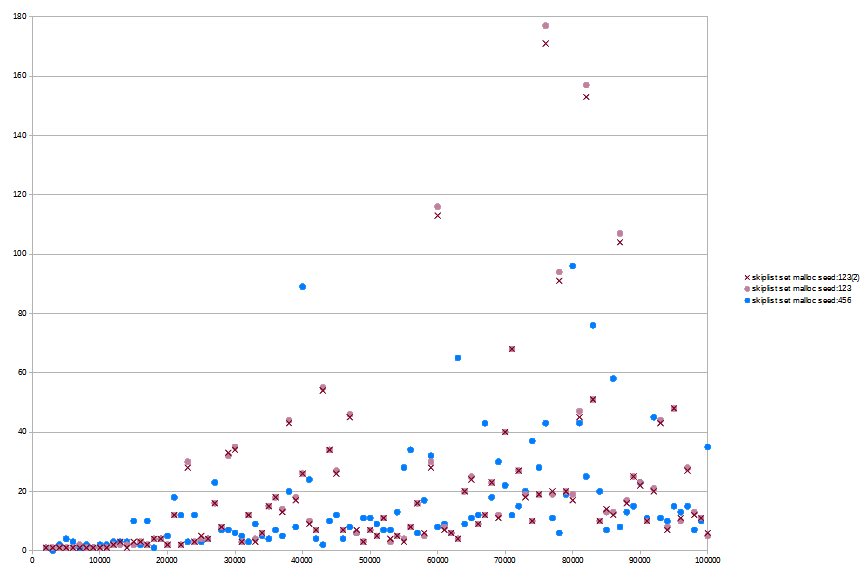
\includegraphics[scale=0.55]{img/diagram_skiplist_seeds}
\label{fig:Img6}

Werden die selben Zufallszahlen verwendet, ist der Aufbau der Listen identisch und das genaue Streumuster stimmt überein. Bei anderen Zufallszahlen unterscheidet sich das genaue Streumuster. Dies belegt die Vermutung, dass die Effizienz einer randomisierten Skip List vom Zufall abhängig ist, je nachdem, wie gut die Liste gebaut wird.

\subsection{Speicherallokation}

In diesem Test wurden die Speicherallokationsmethoden auf Geschwindigkeit analysiert. Es wird die Allocation mittels der c Funktion malloc, einzeln ausgeführt für jeden Knoten; mit dem Nutzen des Speichers in einem globalen Array verglichen. 

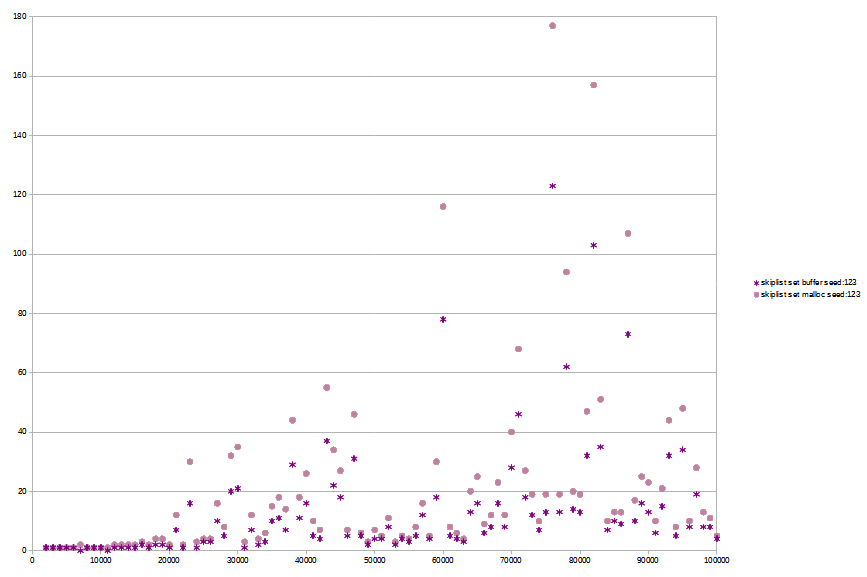
\includegraphics[scale=0.55]{img/diagram_malloc_array_set}
\label{fig:Img7}
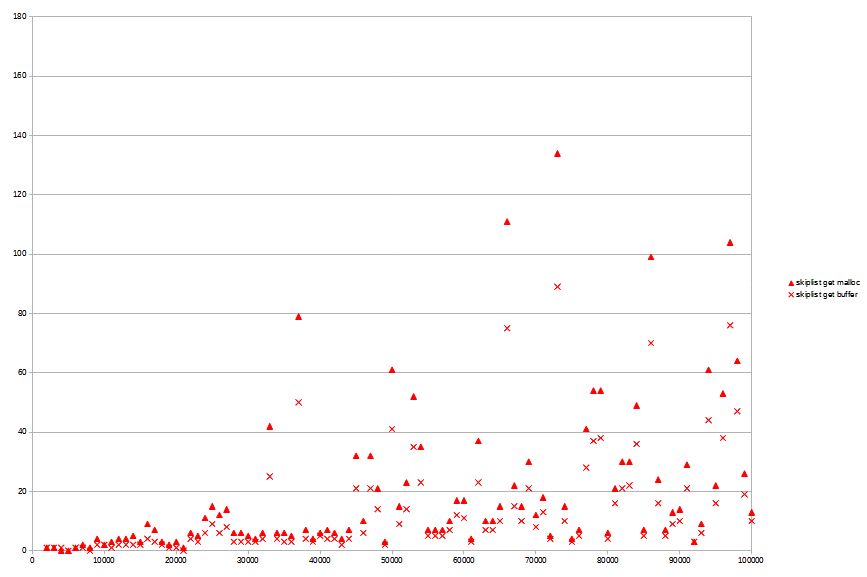
\includegraphics[scale=0.55]{img/diagram_malloc_array_get}
\label{fig:Img8}

Die Methode mit Array scheint beim Einfügen und Suchen deutlich schneller zu sein, woraus man schließen kann, dass dies nicht mit der Zeit, die für das Alloziieren benötigt wird, erklärt werden kann, da dies nur beim Einfügen auftreten würde. Es ist zu vermuten, dass die Array Methode vorteilhaft den Cache ausnutzt, da die Elemente und Knoten in der Nähe voneinander liegen und daher beim Lesen eines Elements oder Knotens auch benachbarte mit gecached werden. 

\section{Fazit}
Die Skip List ist eine \(O(log(n))\) Zeitkomplexe Datenstruktur, jedoch liegen die Knoten und Elemente verstreut über den Speicher. Daher werden, im Gegensatz zu einer Hashmap, welche die selbe Funktionalität, auch \(O(log(n))\) aufweist, die modernen Caches nicht effizient ausgenutzt. Aus diesem Grund sollte die Skip List nicht mehr verwendet werden.

\bibliographystyle{alpha}
\bibliography{quellen}

\newpage
\section{Eidesstattliche Erklärung}
Ich versichere, dass ich diese Arbeit selbstständig verfasst und keine anderen Hilfsmittel als
die angegebenen benutzt habe. Die Stellen der Arbeit, die anderen Werken dem Wortlaut oder
dem Sinn nach entnommen sind, habe ich in jedem einzelnen Fall unter Angabe der Quelle
als Entlehnung kenntlich gemacht. Diese Versicherung bezieht sich auch auf die bildlichen
Darstellungen.\\ \\ \\

17.10.2021 \hfill Fabian Bär

\begin{tikzpicture}[remember picture,overlay]
    \node[xshift=-48mm,yshift=-70mm,anchor=north west] at (current page.north east){
    
\includegraphics[width=25mm]{img/untaschrift}};
\end{tikzpicture}


\end{document} 
